\section{Faulted 3-phase network (3)}
Selecting Base values from generator specification
\begin{align}
    \textrm{Base\_S} & = \SI{12.5}{MVA}                                                         \\
    \textrm{Base\_V} & = \SI{13.3}{kV}                                                          \\
    \textrm{Base\_I} & = \frac{12.6\times 10^6}{\sqrt{3}\times 13.3\times 10^3} = \SI{542.6}{A} \\
    \textrm{Base\_Z} & = \frac{13.3\times 10^3}{542.6} = \SI{24.512}{\ohm}
\end{align}
Per unit values:
\begin{align}
    \SI{12.5}{MVA}    & = \SI{1}{pu,S} \\
    \SI{13.3}{kV}     & = \SI{1}{pu,V} \\
    \SI{542.6}{A}     & = \SI{1}{pu,A} \\
    \SI{24.512}{\ohm} & = \SI{1}{pu,Z}
\end{align}
Per unit conversions. For the motor:
\begin{align}
    \frac{10}{12.5}            & = \SI{0.8}{pu,S}          \\
    \frac{3.3}{13.3}           & = \SI{0.248}{pu,V}        \\
    0.28 \cdot \frac{12.5}{10} & = \SI{0.35}{pu,reactance}
\end{align}
For the transformer:
\begin{align}
    \frac{0.75}{12.5}            & = \SI{0.06}{pu,S}           \\
    0.021\cdot \frac{12.5}{0.75} & = \SI{0.35}{pu,resistance}  \\
    0.013\cdot \frac{12.5}{0.75} & = \SI{0.2167}{pu,reactance}
\end{align}
For Line 1:
\begin{align}
    \frac{0.2}{24.512}  & = \SI{0.0137}{pu,resistance} \\
    \frac{0.45}{24.512} & = \SI{0.031}{pu,reactance}
\end{align}
For Line 2:
\begin{align}
    \frac{1.2}{24.512} & = \SI{0.0827}{pu,resistance} \\
    \frac{2.2}{24.512} & = \SI{0.1516}{pu,reactance}
\end{align}
At location A, we can write out the impedance values.
\begin{figure}[H]
    \centering
    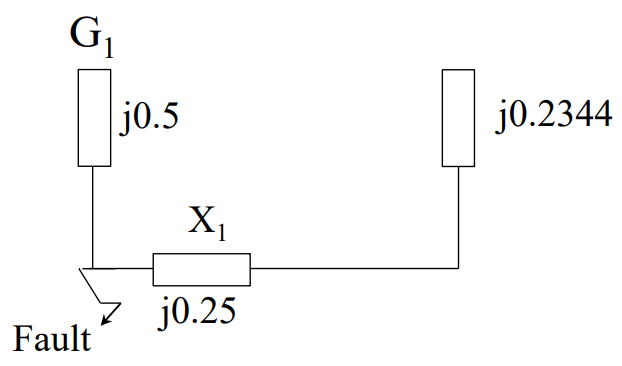
\includegraphics[width = 0.9\textwidth]{img/figure19.jpg}
    \caption{Impedance values for fault A.}
    \label{fig:q5-1}
\end{figure}
\begin{gather}
    \textrm{MVA Fault level} = \frac{25}{\sqrt{0.0069^2 + 0.0805^2}} = \SI{309.4}{MVA}\\
    \textrm{Fault current} = \frac{0.5426}{\sqrt{0.0069^2 + 0.0805^2}} = \SI{6.715}{kA}
\end{gather}
At location B, we can write out the impedance values.
\begin{figure}[H]
    \centering
    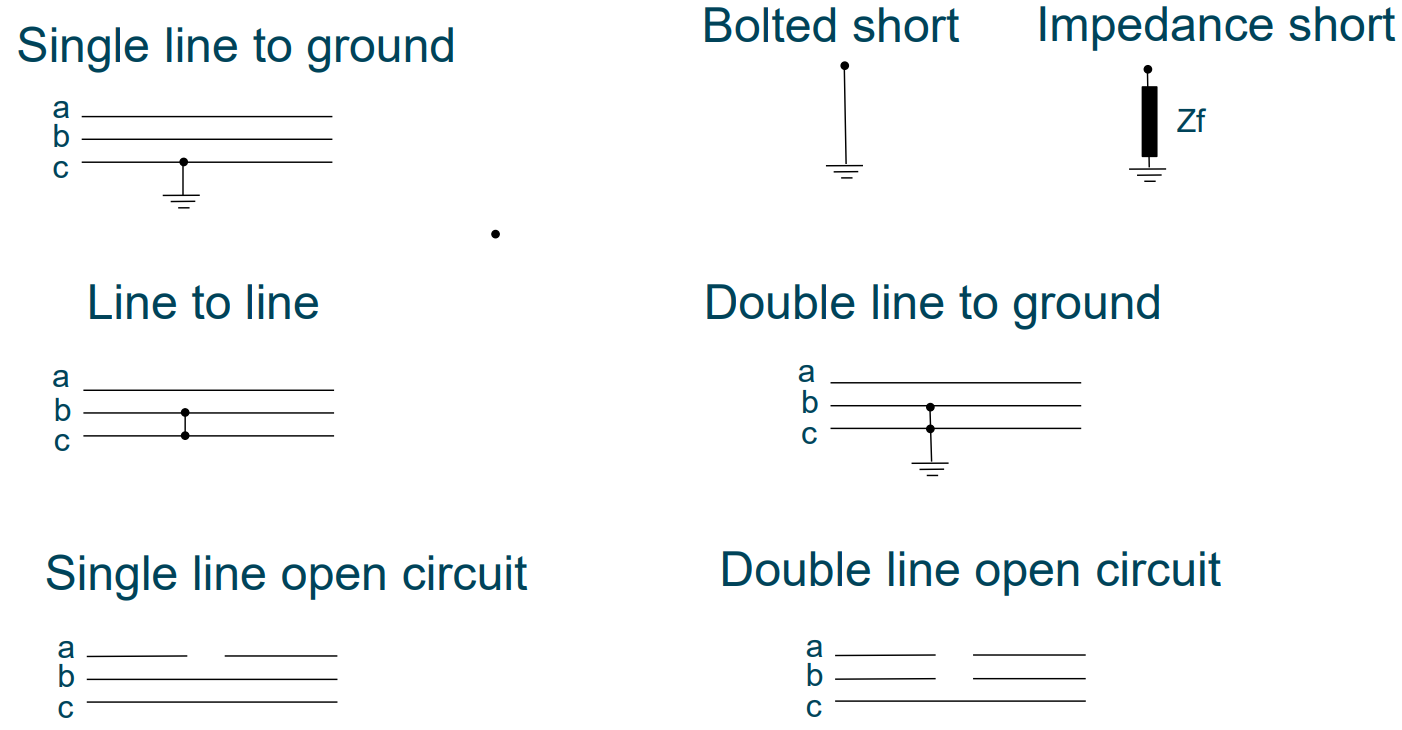
\includegraphics[width = 0.9\textwidth]{img/figure20.jpg}
    \caption{Impedance values for fault B.}
    \label{fig:q5-2}
\end{figure}
\begin{gather}
    \textrm{MVA Fault level} = \frac{25}{\sqrt{0.5223^2 + 0.06004^2}} = \SI{31.3}{MVA}\\
    \textrm{Fault current} = \frac{542.6}{\sqrt{0.5223^2 + 0.6004^2}} = \SI{682}{A}
\end{gather}